\documentclass[a4paper,11pt]{article}

\usepackage{draftwatermark}
\usepackage{amsmath}
\usepackage{authblk}
\usepackage{graphicx}
\usepackage[export]{adjustbox}

\SetWatermarkLightness{0.75}
\SetWatermarkScale{4}

\usepackage{nomencl}
\makenomenclature

\begin{document}
	
\title{Simplified stress analysis of conventional fibrous composite laminates subjected to in-plane loads}
\author{Gustavo Baños Lapuente}
\affil{Airbus Defence and Space, Stress Methods and Optimization}
\renewcommand\Affilfont{\itshape\small}
%\date{\today}
\date{April 11, 2020}
\maketitle


\begin{abstract}
	A simplified methodology for calculating the strain level in a fibrous composite laminate subjected to in-plane loads, provided it complies with conventional design rules and is built from the legacy base of angles 0\textdegree, ±45\textdegree{} and 90\textdegree, is presented, and used, combined with the \emph{Maximum Truncated Strain} criterion, to predict approximately the strength of the laminate.
\end{abstract}


\section{Introduction}

Predicting the ultimate strength of fibrous composite laminates is one of the most significant problems for working efficiently with this kind of materials. A problem which has not been definitively solved indeed, even the combination of Finite Elements Analysis and progressive failure criteria is showing an enormous potential, being one of the most popular topic of research on structural materials along past years.
\\

However, yet nowadays, the extensive use of sophisticated numerical methodologies can be still unpractical in many circumstances for the daily work of a stress engineer, in particular in the aerospace industry. Under these circumstances (pre-sizing, optimization, tests preparation...) the fast and explicit solutions offered by classical handbooks and literature, combined with the internal loads analysis performed with global Finite Elements Models, and even with the handicap of that limited accuracy, prevail as the battle horse along many phases of the design process of airframes. 
\\

The purpose of this paper is to present a simplified methodology to calculate the strain in a laminate (and its conforming plies) under static in-plane loads, when laminate is built using the traditional base of angles (0\textdegree, ±45\textdegree{} and 90\textdegree) following good design practices (balanced, symmetric, ...), in order to predict, approximately, its strength in a later step. It is admitted that this method is merely an adaptation, to this specific work scenario, of available \emph{Classical Laminate Theory} and pre-existing failure theories, and not really an original work. Its merit, if any, is precisely the explicit simplifications done. 
\\


\begin{figure}[h!]
	\centering
	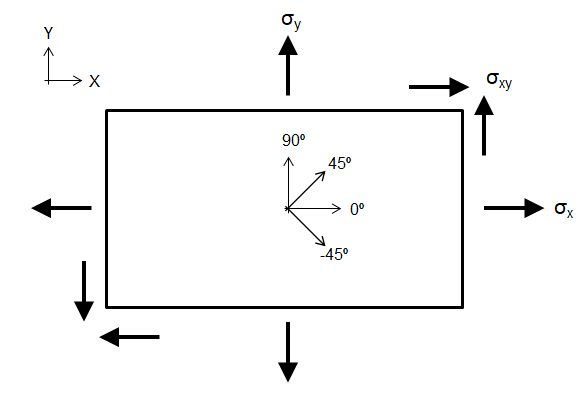
\includegraphics[width=1\textwidth]{fig1_laminate_axis.png}
	\caption{Reference axis system for laminate, plies and loads}
	\label{fig:axis}
\end{figure}


\section{Analysis method}

As noted above, the laminate considered shall follow  good design practices (balanced, symmetric, ...) and be constructed using the legacy base of angles 0\textdegree, ±45\textdegree{} and 90\textdegree{} for its stacking sequence. Without loss of generality (for the in-plane/membrane analysis), a laminate of this kind can be defined by its thickness and the proportions of plies at  0\textdegree, ±45\textdegree{} and 90\textdegree{} directions.

$$w_{0} = n_{0} / n$$
$$w_{45} = n_{45} / n$$
$$w_{90} = n_{90} / n = 1 - w_{0} - w_{45} $$
\\

\subsection{Stiffness and elastic moduli of the laminate}

In a first step of the analysis, the stiffness of the laminate shall be calculated for later stating the basic equation of the \emph{Classical Laminate Theory}. The reduced stiffness matrix of the orthotropic ply (or the quasi-orthotropic laminate) has the shape:

\begin{equation*}
[Q] =
\begin{bmatrix}
Q_{11} & Q_{12} & 0 \\ 
Q_{12} & Q_{22} & 0 \\ 
0      & 0      & Q_{66}    
\end{bmatrix}
\end{equation*}
\\

From Jones' page 72 (Ref. \cite{Jones}), the relationships between reduced stiffness of the lamina (reference is 0\textdegree{} material, or X-laminate, direction) and the material engineering 
constants (elastic moduli) can be expressed as:

	$$	Q^{0}_{11} = E_{1} / (1 - \nu_{12} \cdot \nu_{21})	
		\qquad \qquad	\nu_{12} / E_{1} = \nu_{21} / E_{2}	$$
	$$	Q^{0}_{22} = E_{2} / (1 - \nu_{12} \cdot \nu_{21})	$$
	$$	Q^{0}_{12} = \nu_{12} E_{2} / (1 - \nu_{12} \cdot \nu_{21}) =
	\nu_{21} E_{1} / (1 - \nu_{12} \cdot \nu_{21})	$$
	$$	Q^{0}_{66} = G_{12}	$$
\\

From the same reference, Jones' page 77, it is possible to get the reduced stiffness, referred to the global laminate axis system, also for the plies-pairs at +45\textdegree/-45\textdegree{} as:

	$$	Q^{45}_{11} = Q^{45}_{22} = 0.25 \cdot [Q^{0}_{11} + 2 \cdot (Q^{0}_{12} + 2 \cdot Q^{0}_{66}) + Q^{0}_{22} ]	$$
	$$	Q^{45}_{12} = 0.25 \cdot (Q^{0}_{11} + Q^{0}_{22} - 4 \cdot Q^{0}_{66}) + 0.5 \cdot Q^{0}_{12}	$$
	$$	Q^{45}_{66} = 0.25 \cdot (Q^{0}_{11} + Q^{0}_{22} - 2 \cdot Q^{0}_{12} - 2 \cdot Q^{0}_{66}) + 0.5 \cdot Q^{0}_{66}	$$
	$$	Q^{45}_{16} = Q^{45}_{26} = 0 \qquad \mbox{(provided +45\textdegree{} and -45\textdegree{} plies come in pairs)}	$$
\\

Plies at 90\textdegree{} shall have the same stiffness matrix as 0\textdegree{} plies but interchanging $Q_{11}$ and $Q_{22}$ terms.
\\

Then the reduced stiffness matrix for the laminate can be obtained summing the previous matrices weighted by the respective proportions of the plies at 0\textdegree, ±45\textdegree{} and 90\textdegree{} directions within the laminate:

	$$	[Q] = w_{0} \cdot [Q]^{0} + w_{45} \cdot [Q]^{45} + w_{90} \cdot [Q]^{90}	$$
\\

Note that the apparent elastic moduli of the laminate can be derived from the resulting $[Q]$ matrix (equal to $[A]/t$) using the expressions presented above for the ply, but expressed as $E_{i} = f(Q_{ij})$.

	$$	\nu_{xy} = Q_{12} / Q_{22}		$$
	$$	E_{x} = (Q_{12})^{2} / Q_{22}	$$
	$$	E_{y} = (Q_{12})^{2} / Q_{11}	$$
	$$	G_{xy} = Q_{66}					$$
\\


\subsection{Strain in laminate and its plies}

The mid-plane strain is obtained using the Classical Lamination Theory from the applied loads (in-plane forces per unit width)
modifying slightly the familiar expression $[N] = [A] [\varepsilon]$, for dealing with apparent stresses instead of plate forces, as:

\begin{equation*}
	\begin{bmatrix}
		\sigma_{x} \\ 
		\sigma_{y} \\ 
		\sigma_{xy} 
	\end{bmatrix}
	= [Q] 
	\begin{bmatrix} 
		\varepsilon_{x} \\ 
		\varepsilon_{y} \\ 
		\gamma_{xy} 
	\end{bmatrix}
	\qquad \Rightarrow \qquad
	\begin{bmatrix} 
		\varepsilon_{x} \\ 
		\varepsilon_{y} \\ 
		\gamma_{xy} 
	\end{bmatrix}
	= [Q]^{-1} 
	\begin{bmatrix} 
		\sigma_{x} \\ 
		\sigma_{y} \\ 
		\sigma_{xy} 
	\end{bmatrix}
\end{equation*}
\\

Strains  $\varepsilon_{x}$, $\varepsilon_{y}$, $\gamma_{xy}$ can be obtained from expression above, where $\varepsilon_{x}$ and $\varepsilon_{y}$ are equal to the strain at 0\textdegree{} and 90\textdegree{} plies respectively. The strain levels at 45\textdegree{} plies can be obtained also from values
of $\varepsilon_{x}$, $\varepsilon_{yx}$, $\gamma_{xy}$ and the appropriate transformation equations (see Jones' 2.73). Or, expressed via the engineering constants, without the matrix notation:

	$$	\varepsilon_{0} = \varepsilon_{x} = \sigma_{x} / E_{x} - \nu_{xy} \cdot \sigma_{y} / E_{x} 	$$
	$$	\varepsilon_{90} = \varepsilon_{y} = \sigma_{y} / E_{y} - \nu_{xy} \cdot \sigma_{x} / E_{x}	$$
	$$	\gamma_{xy} = \sigma_{xy} / G_{xy}	$$
	$$	\varepsilon_{45} = (\varepsilon_{x} + \varepsilon_{y} + \gamma_{xy}) / 2	$$
	$$	\varepsilon_{-45} = (\varepsilon_{x} + \varepsilon_{y} - \gamma_{xy}) / 2	$$
\\

\subsection{Strength of the laminate}

The selected failure criterion for the laminate is the \emph{Maximum Truncated Strain} criterion proposed by Hart-Smith and suggested
by the CMH-17 Vol. 3 Chpt. 8 (Ref. \cite{CMH-17}). Its simplicity is consistent with the motivation of this method. Nevertheless, it is strongly 
recommended that the allowable strain values used for the analysis do not rely exclusively on the tests results for the 
uni-directional laminate.
\\

For plies at 0\textdegree/90\textdegree{} and for plies at +45\textdegree/-45\textdegree{} it must be checked that:

	$$ 	\varepsilon_{1c} < \varepsilon_{1} < \varepsilon_{1t} 	$$
	$$ 	\varepsilon_{1c} < \varepsilon_{2} < \varepsilon_{1t} 	$$
	$$ 	|\varepsilon_{1} - \varepsilon_{2}| < (1+\nu_{12})  \cdot  max(\varepsilon_{1t}, \varepsilon_{1c}) 	$$
\\

Material allowable values to be use in expressions above:
\begin{itemize}
\item Tension allowable strain $\varepsilon_{1t}$ shall be preferably corrected with results available from plain strength tests in multi-angular
laminates, e.g. in the quasi-isotropic (45/-45/90/0)$_{N}S$ \footnote{Using the allowable tension strain obtained from the tension test on the QI laminate might NOT be conservative for laminates with less that than 25\% plies in tension load direction}
\item Compression allowable strain $\varepsilon_{1c}$ can be directly obtained from the longitudinal compression test in the UD laminate as $F_{1c}/E_{1}$ 
\item For bi-axial fabric materials ($E_{1} = E_{2}$), instead of the Poisson's ratio of the material $\gamma_{12}$, use directly a value of 0.3 (i.e. treat the
fabric ply as a cross-ply 0/90 sublaminate made of a fictitious UD tape material with the same allowable strains)
\\
\end{itemize}


\section{Conclusions}

This paper presented a simple and fast method for checking the plain strength of composite laminates (following the traditional design rules) under static in-plane loads.
\\

An implementation of this methodology is available in a Microsoft Excel spreadsheet named \emph{ANCOsheet}. The distribution and use of this software is permitted under the terms of the BSD License 2.0. The following figures exemplify the use of this spreadsheet for calculating the laminate elastic moduli and for predicting its plain strength. Material data in this example are taken from the NIAR qualification tests report for the Hexcel AS4/8552 UD pre-preg CFRP material (Ref. \cite{AS4/8552}): mean values at RTD conditions, converted to the SI units (MPa), Young's modulus (see Figure \ref{fig:moduli}) as the average of the values from tension and compression results in UD tests (rounded to 2-3 significant digits and, in longitudinal direction, normalized with the nominal ply thickness), allowable strengths according to recommendations in previous section ($\varepsilon_{1t}$ from the QI laminate tension strength, $\varepsilon_{1c}$ from the longitudinal compression strength). Notice the presented static margins (the Reserve Factors indeed, $RF$ values in Figure \ref{fig:strength}) correspond to the unnotched plain strength of the (50/40/10) \emph{hard} laminate and show reasonably conservative predictions. 
\\

\begin{figure}[h!]
	\centering
	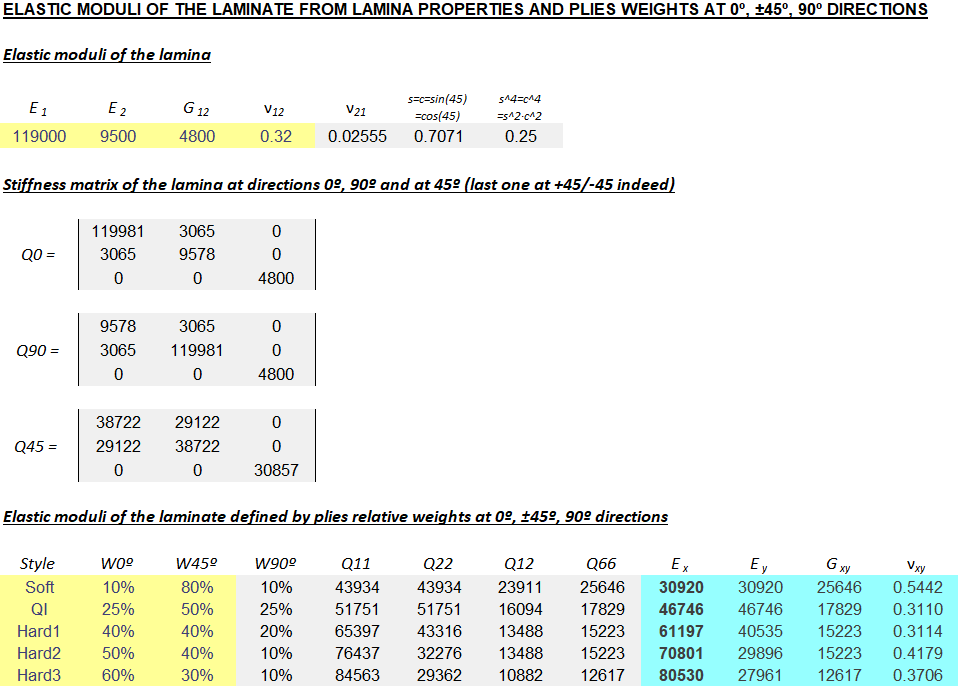
\includegraphics[width=\linewidth, frame]{fig2_anchosheet_moduli.png}
	\caption{Apparent elastic moduli of Hexcel AS4/8552 calculated with \emph{ANCOsheet}}
	\label{fig:moduli}
\end{figure}

\begin{figure}[h!]
	\centering
	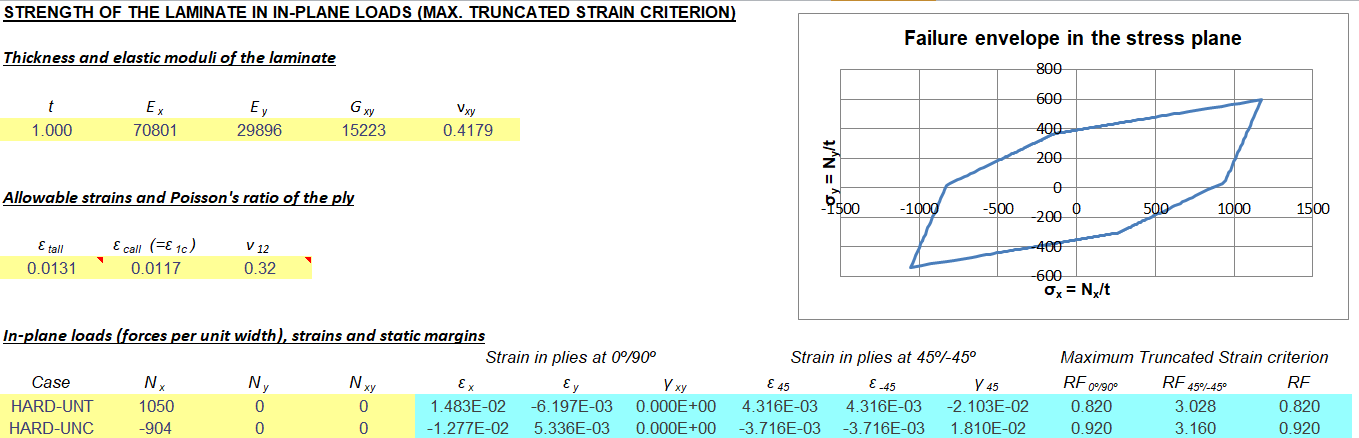
\includegraphics[width=\linewidth, frame]{fig3_anchosheet_strength.png}
	\caption{Plain strength of a \emph{hard} (50/40/10) laminate made of Hexcel AS4/8552 predicted by \emph{ANCOsheet}}
	\label{fig:strength}
\end{figure}

Note that the laminate/plate failure due to loss of stability (buckling) under compression or shear loads is out of the scope of this method but shall have to be checked anyway.
\newpage


\nomenclature{$E_{1}$}{Elastic modulus of the ply material in longitudinal direction}
\nomenclature{$E_{2}$}{Elastic modulus of the ply material in transverse direction}
\nomenclature{$G_{12}$}{In-plane shear modulus of the ply material}
\nomenclature{$\nu_{12}$}{Poisson's ratio of the ply material}
\nomenclature{$1$}{As supscript, local longitudinal direction of the ply}
\nomenclature{$2$}{As supscript, local transverse direction of the ply}
\nomenclature{$x$}{As supscript, global longitudinal direction of the laminate, typically matching material reference direction 0\textdegree}
\nomenclature{$y$}{As supscript, global transverse direction of the laminate}
\nomenclature{$N$}{Internal loads in laminate (force per unit width)}
\nomenclature{$\sigma$}{Stress (note the apparent stress in the laminate is $[\sigma] = (1/t) \cdot [N]$)}
\nomenclature{$\varepsilon$}{(Axial) strain}
\nomenclature{$\varepsilon_{1t}$}{Allowable tension strain}
\nomenclature{$\varepsilon_{1c}$}{Allowable compression strain}
\nomenclature{$\gamma$}{Engineering shear strain}
\nomenclature{$[A]$}{In-plane stiffness matrix of the laminate}
\nomenclature{$[Q]$}{Reduced stiffness matrix of the laminate/ply, $[Q] = (1/t) \cdot [A]$}
\nomenclature{$t$}{Thickness of the laminate}
\nomenclature{$n$}{Total number of plies in the laminate}
\nomenclature{$n_{0}$}{Number of plies oriented at 0\textdegree{} direction}
\nomenclature{$n_{45}$}{Number of plies oriented at ±45\textdegree{} directions}
\nomenclature{$n_{90}$}{Number of plies oriented at 90\textdegree{} direction}
\nomenclature{$w_{0}$}{Proportion of plies oriented at 0\textdegree{} direction}
\nomenclature{$w_{45}$}{Proportion of plies oriented at ±45\textdegree{} directions}
\nomenclature{$w_{90}$}{Proportion of plies oriented at 90\textdegree{} direction}
\nomenclature{$CFRP$}{Carbon Fibre Reinforced Polymer}
\nomenclature{$SI$}{International Units System}
\nomenclature{$FEM$}{Finite Elements Model}
\nomenclature{$RF$}{Reserve Factor, i.e. ration between allowable load and applied load}
\nomenclature{$UD$}{Uni-Directional (material or laminate)}
\nomenclature{$QI$}{Quasi-Isotropic, referred to a kind of laminates, made typically of packages of the (45/-45/90/0) sub-laminate}

\printnomenclature


\begin{thebibliography}{99}
	\bibitem{Jones} MECHANICS OF COMPOSITE MATERIALS, 2nd Edition, by R. M. Jones
	\bibitem{CMH-17} COMPOSITE MATERIALS HANDBOOK (CMH-17), Edition 2012, by the FAA/SAE
	\bibitem{AS4/8552} Hexcel 8552 AS4 Unidirectional Prepreg at 190 gsm \& 35\% RC Qualification Material Property Data Report (NCAMP Test Report Number: CAM-RP-2010-002 Rev A), May 2011, by the NIAR
\end{thebibliography}	


\end{document}
